%-----------------------------------------------------------------------------%
\chapter{\babEmpat}
\label{chap:babEmpat}
%-----------------------------------------------------------------------------%

Pada bab ini dijelaskan hasil evaluasi dan analisis dari penelitian ini.

%-----------------------------------------------------------------------------%
\section{Evaluasi}
%-----------------------------------------------------------------------------%

Kedua eksperimen di atas akan dilakukan pada \textit{notebook} dengan sistem operasi \textit{Ubuntu 15.04 64-bit}, prosesor \textit{Intel Core i7 5500U} (\textit{dual cores}), RAM DDR3 8 GB dan penyimpanan SSD 250 GB. Program yang digunakan untuk melakukan eksperimen tersebut adalah \verb|classifier.py|


In this research, we report two experiments. The first one shows the performance comparison of four classifiers in selecting valid triples from given candidates. While the second one shows the scalability of our system (using the best classifier) extracting triples from documents (unannotated). Both experiments are run on an Ubuntu 15.04 64-bit, Intel Core i7 5500U (dual cores), DDR3 8 GB RAM, SSD 250 GB machine.

In the first experiment, we chose four classifiers each representing unique characteristics: 

\begin{enumerate}
\item Linear Logistic Regression\cite{fan2008liblinear} (linear model)
\item Polynomial Support Vector Machine (SVM)\cite{chang2011libsvm} (nonlinear model)
\item Multi-Layer Perceptron (MLP)\cite{hinton1989connectionist} with 2 hidden layers (20 and 10 ReLU\cite{nair2010rectified} neurons)
\item Random Forest\cite{wasserman2015grid} (ensemble decision trees)
\end{enumerate}
  
We use the manually annotated triple selector dataset described in Section \ref{Triple Candidates Generator} to cross-validate\cite{kohavi1995study} (k-Fold with $k=3$) the four classifiers. Since open IE systems requires both precision and recall\cite{angeli2015leveraging}, we choose F1 score to determine the best classifier for triple selector. The result of this experiment is shown by Figure \ref{fig_models_performance} and Table \ref{table_models_performance} where Random Forest achieves the highest F1 score 0.58.

\begin{figure}
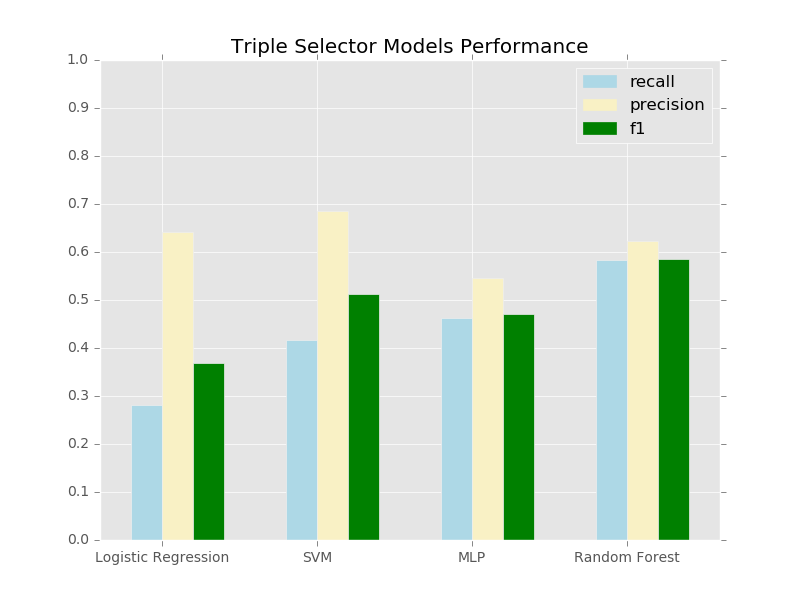
\includegraphics[scale=0.4]{../images/models_performance.png}
\caption{Triple selector models performance comparison chart}
\label{fig_models_performance}
\end{figure}

\begin{table}[!t]
\renewcommand{\arraystretch}{1.5}
\caption{Triple selector models performance}
\label{table_models_performance}
\centering
\begin{tabular}{l r r r}
\hline
\textbf{Model} & \textbf{P} & \textbf{R} & \textbf{F1} \\
\hline
Logistic Regression & 0.64 & 0.28 & 0.36 \\
SVM & \textbf{0.68} & 0.41 & 0.51 \\
MLP & 0.54 & 0.46 & 0.47 \\
Random Forest & 0.62 & \textbf{0.58} & \textbf{0.58} \\
\hline
\end{tabular}
\end{table}

In the second experiment, we evaluate the performance of our system by extracting triples from three documents with different number of sentences, measuring the total execution time and calculating the average execution time per sentence. The result in Table \ref{table_system_extraction_time} shows that the lowest execution time (or fastest execution time) is 0.014 seconds when processing document of 5,593 sentences.

\begin{table}[!t]
	\renewcommand{\arraystretch}{1.5}
	\caption{System end-to-end extraction time}
	\label{table_system_extraction_time}
	\centering
	\begin{tabular}{l p{1.2cm} p{1.2cm} p{1.2cm}}
		\hline
		\textbf{Sentences} & \textbf{Triples Extracted} & \textbf{Total Time (s)} & \textbf{Time per Sentence (s)} \\
		\hline
		2 & 7 & 6.1 & 0.800 \\
		138 & 429 & 11.3 & 0.082 \\
		5,593 & 19,403 & 78.6 & 0.014 \\
		\hline
	\end{tabular}
\end{table}


%-----------------------------------------------------------------------------%
\section{Analisis}
%-----------------------------------------------------------------------------%

The first experiment shows that all classifiers are still having problem learning the pattern of triples when cross-validated using $k=3$ which means two thirds of our dataset is insufficient to cover the patterns in other one third part. The dataset also suffers unbalance 1:11 ratio of positive and negative samples which is caused by lack of efficiency in triple candidates generator. To solve this issue, we plan to annotate more sentences to increase the coverage and improve the efficiency of triple candidates generator. The low performance of linear logistic regression indicates that this problem is not linearly separable. The random forest performs better than other nonlinear models (SVM and MLP) because it is easily tuned to balance the precision and recall by changing the number and the depth of decision trees.

We are also aware that the heuristics used in triple candidates generator and token expander are still limited to explicit pattern. For instance, triple candidate generator can not extract relations \textit{(kecamatan Kejajar, terletak di, Jawa Tengah)} and \textit{(Jawa Tengah, terletak di, Indonesia)} from the sentence in Figure \ref{fig_example_io_openie} yet. In the future research, we plan to improve the model to extract implicit patterns while keeping the number of negative candidates. The token expander is having problem in expanding token to implicitly expected clauses such as \textit{"seorang pelatih sepak bola"} from \textit{"seorang pelatih dan pemain sepak bola"} or \textit{"satu buah torpedo"} from \textit{"satu atau dua buah torpedo"}. We expect there will be more patterns that need to be considered in order to properly expand the token so further research on effective model to achieve this is required. Also, in order to properly evaluate the performance of these components, we need to create test datasets for both triple candidates generator and token expander.

Additionally, through the second experiment, we also find that our system average extraction performance is 0.014 seconds/sentence (for 5,593 sentences document) which is still comparable to TextRunner\cite{banko2007open}. Therefore, in contrast to the argument proposed in the related work\cite{banko2007open}\cite{etzioni2011open}, this experiment shows that the heavy linguistic tasks such as dependency parsing doesn't cause performance drawback in big document, assuming the average number of sentences in document do not exceed 5,593.
